%% LaTeX2e class for student theses
%% sections/content.tex
%% 
%% Karlsruhe Institute of Technology
%% Institute for Program Structures and Data Organization
%% Chair for Software Design and Quality (SDQ)
%%
%% Dr.-Ing. Erik Burger
%% burger@kit.edu
%%
%% Version 1.3.2, 2017-08-01


\chapter{Foundations}
\label{ch:Foundations}
In this section, we introduce the necessary foundations for this thesis. In section \ref{sec:The Palladio Component Model}, we present the Palladio Component Model (PCM) and it's models. In section \ref{sec: SEFFs}, we describe briefly the Service Effect Specification (SEFF) model of PCM. In section \ref{sec:Vitruvius}, we present the Vitruvius Framework. In section \ref{sec:Java Model Parser and printer}, we present Java Model Parser and Printer (JaMoPP). In section \ref{sec:Automated Coevolution of Source Code and Software Architecture Models}, we introduce the Coevolution approach \cite{langhammer2015co}. In section \ref{sec:Kieker Monitoring}, we present the Kieker Monitoring Framework. In section \ref{sec:Source Code Model eXtractor}, we give an overview of the reverse-engineering of the approach Source Code Model eXtractor (SoMoX). In section \ref{sec:Continuous Integration of Performance Model}, we bring in the approach Continuous Integration of Performance Model (CIPM). In section \ref{sec:Iterative Performance Model Parameter Estimation Considering Parametric Dependencies}, we summarize the master thesis of Jägers. In the last section \ref{sec:DevOps}, we introduce the development process DevOps.

\section{Eclipse Modeling Framework}
\label{sec:Eclipse Modeling Framework}
Eclipse Modeling Framework (EMF) is a framework, that enable the creation of meta-models based on Ecore. Moreover, EMF provides the following facilities:
\begin{itemize}
\item Source code generation from meta-models. 
\item Generate an instance of eclipse in order to instantiate meta-models and edit them.
\end{itemize}    

\section{The Palladio Component Model}
\label{sec:The Palladio Component Model}
Palladio Component Model (PCM) is a component-based software architecture approach, that can be used to predict and evaluate the performance and the reliability of component-based software systems at design stage. For performance prediction, it makes it possible to analyze the components of the software architectures before implementation and thus it can for example detects bottlenecks, predict response time and predict throughput. For software reliability, PCM specifies metrics like detecting the probability of failures on demand. 

\subsection{Palladio Models}
\label{sec: Palladio Models}
To allow the prediction of the Performance and the reliability of a software system, PCM defines four different roles to create four different models \ref{fig:PCM Models and transformations}. The Repository model, which is created by developers. Developers specify and implement components, interfaces, provided roles, required roles and signatures for the repository. In the context of PCM, a component is by definition a block of software, that can be composed, deployed and customized without requiring the understanding of its internals.  Moreover, the roles in PCM specify the relation between the components and the interfaces. Developers should also specify the internal behavior of the components in term of Service Effect Specification (SEFF). The Assembly model is created by software architects. Software architects use the existing components in repository to create the software system. The allocation model is created by system deployers.  Deployers are responsible for specifying the environment resource, like Servers, CPUs, HDDs and network connection. Afterwards, they decide which assembly can be deployed in which resource. The usage model is created by domain experts. Domain experts provide information about the interaction between the system and the users. Additionally, domain experts can define the relevant critical usage scenarios and the inputs parameters values. 

In the context of this thesis, we will use the information provided by SEFFs. Thus, we will explore the related concepts based on \cite{becker2009palladio} and \cite{koziolek2006parameter}.

\begin{figure}[h]
\centering
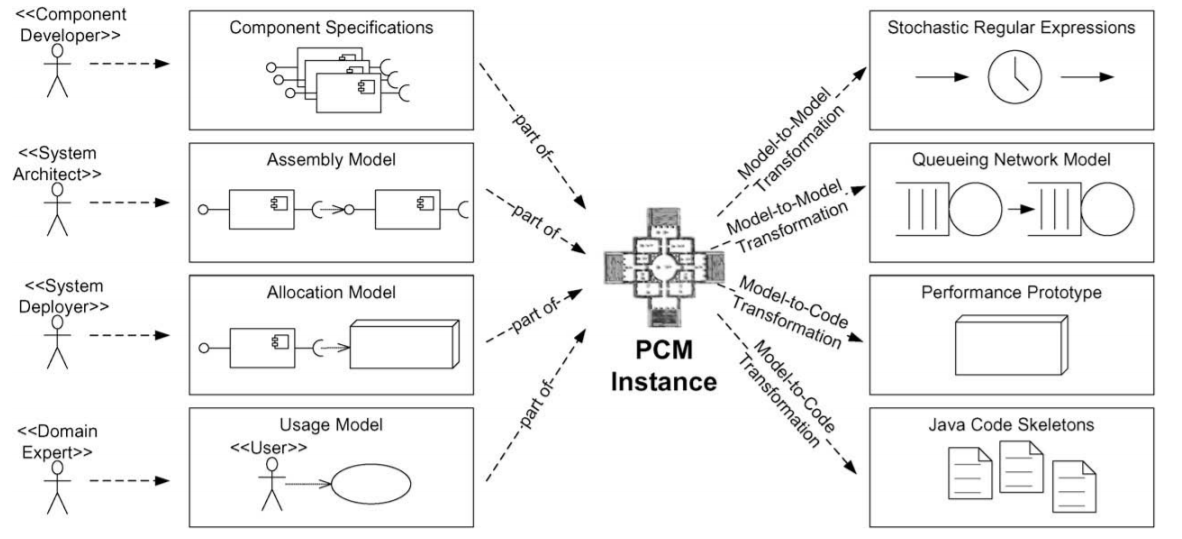
\includegraphics[width=0.9\textwidth]{figures/pcmmodels}
\caption{PCM Models and transformations \cite{reussner2016modeling}}
\label{fig:PCM Models and transformations}
\end{figure}


\subsection{SEFFs}
\label{sec: SEFFs}
Service Effect Specification (SEFF) were firstly presented by \cite{koziolek2006parameter}, which describes like a UML Activity Diagram the control flow of component services. For each provided service, SEFF describes how services in the required interface are called in the provided service. Moreover, as mentioned before, the components in PCM can be used without understanding their internals and thus as a black box. However, SEFF turns a component to a gray box by describing the behavior of its provided services.
The ResourceDemandingServiceEffectSpecifaction (RDSEFF) used in PCM to predict the performance, is an extension of SEFF. RDSEFF offers the possibility to add performance inputs values associated to each activity of SEFF. Moreover, to each component provided service, developers can specify a RDSEFF in order to describe how the service uses the hardware/software resources and how it calls the component's required services. 
In the rest of this thesis, we will indicate RDSEFF as SEFF in order to avoid ambiguity. The principal elements of SEFF will be explored in the following. SEFF includes the so called ExternalCallActions which present the call of a required Service within the SEFF. InternalActions are used within SEFF to abstract the internal computation of the component. Moreover, an internal action can be defined as a set of successive instruction, that do not include any external call from other components. LoopActions within SEFF are specified to indicate the number of times the sub control flow within the loop is going to be executed. BranchActions models the branches within the control flow. The execution of a branch can be decided either on an input parameter or a probability. InternalActionActions refers to the internal behavior of a component, that can be only used by the services of this component. 
To have a better understanding of these concepts, we put them together in an example \ref{fig:Example of source code and SEFF}, which depicts on the right hand the source code and on the left hand the corresponding SEFF model. The implementation of the Service service() starts with an internal call of an inner method. Since the inner method innerMethod1() represent an internal computation and does not make any external call, it is seen an internal action within SEFF. Within the next branch is seen as a BranchAction, because there is a call of the service service1() of the component componentB. In the second branch transition, there is loop, which makes call of the external service service2(), that’s why it’s represented as a LoopAction within the corresponding SEFF. 

\begin{figure}[h]
\centering
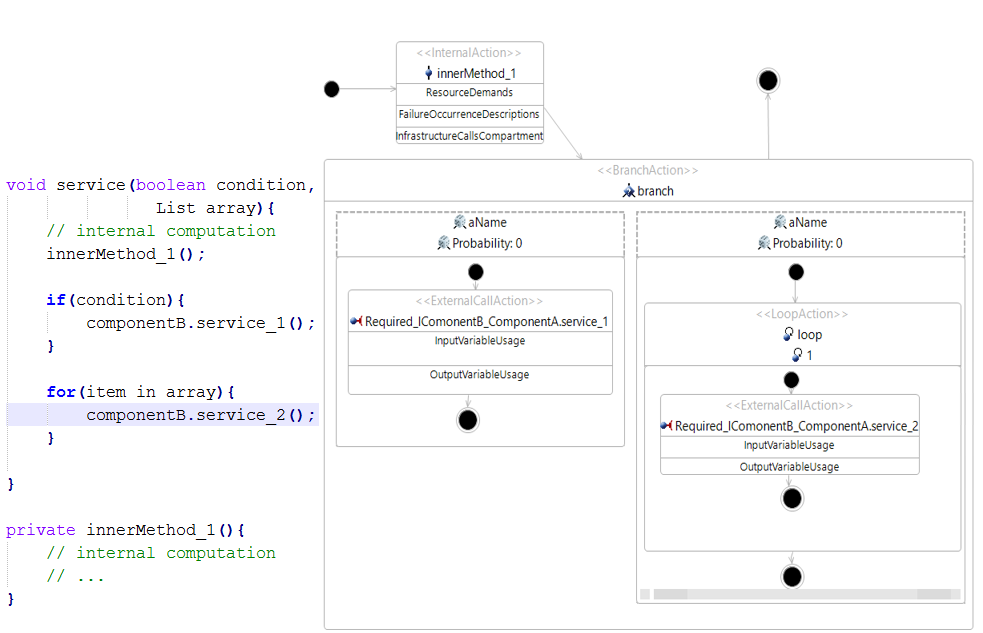
\includegraphics[width=0.9\textwidth]{figures/code_seff}
\caption{Example of source code and SEFF}
\label{fig:Example of source code and SEFF}
\end{figure}


\section{Vitruvius}
\label{sec:Vitruvius}

The Vitruvius approach is a view-based \cite{goldschmidt2012view} engineering approach, which was introduced in \cite{burger2013flexible, kramer2013view}.  Vitruvius can be used to keep the models of a system consistent. In Model Driven Engineering (MDE) \cite{thomas2005erzeugung}, the whole system can be represented by different models that describe different aspects of the system, even the source code of the system is seen as a model. These models can be changed separately and became inconsistent, for example if the source code of a system has changed, the architecture model of the system has to be also updated. In this case, architectures must capture the changes in the source code and update accordingly the associated architecture model. Therefore, Vitruvius performs this task automatically by defining consistency rules that define how the changes in a model must be transformed to another model.

Vitruvius uses views to make access to the models possible. This approach reduces the complexity of dealing with the whole models, because views present only a part of the model. Therefore, developers can focus only on the relevant parts of the system.

Vitruvius defines the so called Virtual Single Underlying Model (VSUM), which contains all information related to a system. VSUM contains the meta-models instances, that are used within a system. Moreover, Vitruvius provides the correspondence meta-model, which offers the possibility to map between correspondent elements of different model, like SEFFs in PCM and methods in Java source code.  

To enable the process of keeping models consistent within Vitruvius, developers should provide and implement two concepts defined by Vitruvius, namely Domains and Application. A Vitruvius Domain represents a defined meta-model in the system and provides information for its use within the Vitruvius framework. Vitruvius Domains can be reused, for example the Domain of Java meta-model can always be used in systems that are implemented using java. Vitruvius Applications determine the relation between two Domains. They specify how changes in a Domains meta-model instance should be transformed to the instance of another Domains meta-model instance. Vitruvius Applications can be also reused in many environments, if the are needed.

\subsection{Vitruvius VSUM}
\label{sec:Vitruvius VSUM}
In order to keep models instances consistent, Vitruvius approach uses the so-called Virtual Single Underlying Model (VSUM) which contains all information that represents the system Figure \ref{fig:vitruv_vsum}. The models in VSUM are accessible using views. Views are instances of view types and they can be used to manipulate model instances. Moreover, there are two kinds of view types, namely projectional view types or combining view types \cite{burger2013flexible}. Projectional view types allows to show information from one meta-model solely. Combining view types can be used to show information from diverse meta-models.

Models consistency in Vitruvius can be preserved using Consistency preservation rules. They describe how changes in one model should be transferred into changes in another model. Moreover, the Consistency Preservation Process uses these rules to create the models transformation that preserves the consistency.


\begin{figure}[h]
\centering
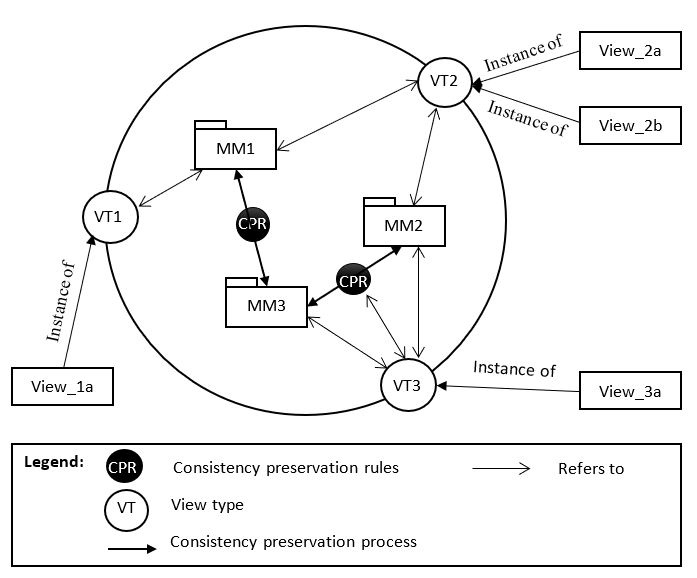
\includegraphics[width=0.9\textwidth]{figures/vitruv_vsum}
\caption{Overview of the Vitruvius VSUM and how model instances can be kept consistent}
\label{fig:vitruv_vsum}
\end{figure}

\subsection{Correspondence Meta-model}
\label{sec:Correspondence Meta-model}
The Correspondence Metamodel (CMM) is used within Vitruvius in order to describe the corresponding elements of two meta-models. Moreover, Vitruvius one instance of CMM can be used for each Vitruvius application. A Vitruvius application can have one or many meta-models instances.  In our approach, we use one CMM instance which has been created and used in the Coevolution approach. Furthermore, for the process of probes generation we will use the existing information in this instance that have been saved the Coevolution approach and add new information to it by extending the Coevolution approach.

Figure \ref{fig:correspondence_model} shows the Vitruvius Correspondence Meta-model. It's basically composed from two classes. The root class Correspondences contains the list of Correspondence. The class Correspondence is composed from two list of identifier references. The first list contains identifiers that reference models in one meta-model, while the second list contains identifiers that reference models in the other meta-model.

CMM is a generic and can be used for diverse meta-models. Therefore, in order to identify an element, the reference in the Correspondence has to be unique because only one concrete element needs to be identified for a given ID. For this purpose, the CMM uses the so-called Temporarily Unique Identifier (TUID) mechanism. TUID is a string that can identifies an element. It has to be calculated based on the properties of the element that it represents. The TUID is also used when an element needs to be retrieved from the correspondence model.    

\begin{figure}[h]
\centering
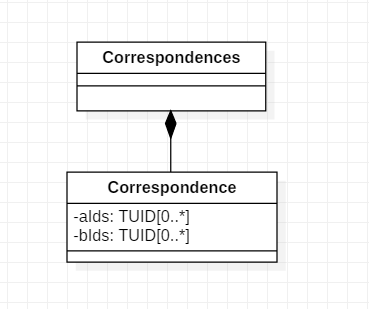
\includegraphics[width=0.6\textwidth]{figures/correspondence_model}
\caption{The Correspondence Meta-model of the Vitruvius Framework}
\label{fig:correspondence_model}
\end{figure} 

\section{Java Model Parser and printer}
\label{sec:Java Model Parser and printer}

Java Model Parser and Printer (JaMoPP) \cite{heidenreich2009closing} is a parser and printer for the Java language. JaMoPP defines a complete meta-model for the Java language based on the meta modeling language Ecore \cite{steinberg2008emf}. JaMoPP parser allows to parse a Java source code into a Java model, and the JaMoPP printer allows to print a Java model into Java source code. JaMoPP can convert Java source code into an EMF model, which can be manipulated using model driven techniques, like models transformation. Using JaMoPP, we can for example, parse a Java file, which contains Java source code, add new Java statements after or before an existing statement and print back the changes in the Java source code file. The creation of JaMoPP is based on EMFText \cite{heidenreich2009derivation}, which allows to define text syntax for languages described by an Ecore meta-model. 


\section{Automated Coevolution of Source Code and Software Architecture Models}
\label{sec:Automated Coevolution of Source Code and Software Architecture Models}
The approach of co-evolution of source code and component-based software architecture presented in \cite{langhammer2015co, langhammer2017automated} is based on the platform Vitruvius present above. It gives developers and architectures the possibility to keep the architecture and the source code of a software system consistent. The Consistency in this approach is kept in both directions, that means, if developers changed the source code of a system, the corresponding architecture will automatically be changed, and if architectures updated the architecture of the system, the source code will also automatically be updated. The co-evolution approach uses PCM models as architectures models.  Therefore, it describes the behavior of the source code in term of SEFF. Hence, a special objective of the co-evolution approach is to keep incrementally the behavior of the source code consistent with the source code itself. The incremental up-to-date of the behavior model of the source consists of only the part of the SEFF that corresponds to the changes performed in the source code. For example, if the developers update a service S of Component A, only the SEFF of the service S will be reconstructed but not the whole SEFF model of the system. 

The co-evolution approach uses two different concepts to preserve different modes consistent, namely model-driven engineering and change-driven engineering. Moreover, the co-evolution approach uses the concepts of Vitruvius to keep tracks of the models, that represents the system. 

The co-evolution approach considers all involved artifacts as models. Hence, the model-driven engineering is used in this approach as a main concept. In mode-driven engineering, all artifacts of the system are represented by models and the models are centric in the development process. That means, that the source code must be also represented within the co-evolution approach as a model. Therefore, in the case of Java, the co-evolution approach uses JaMoPP to parse the Java source code to a mode, on which the change-driven techniques can be applied, like model to model transformations.

The co-evolution approach uses change-driven engineering in order to reacts on changes, that the users perform on models, especially the architecture model and the source code model. These changes are monitored, converted in a Vitruvius change model and propagated. The propagated changes can be captured and transferred using consistency preservation rules to the target model. The consistency preservation rules are bidirectional and defined between the architecture meta-model and the source code meta-model.

The co-evolution approach was applied to the Palladio Component Model (PCM) as an architecture model and Java source code.  However, the concepts presented in this approach can be applied to other component-based architecture model, like UML component-diagrams, and other object-oriented languages. In the following, we will review the application of the co-evolution approach to PCM and Java source code and the steps, that are required to keep PCM models instances and Java source code consistent. 



Figure  \ref{fig:coevoloution approach} shows the steps, that are used to keep architecture models and the source code consistent:

\begin{itemize}
\item Step (0): users change either the PCM repository, the PCM system or the Java source code.  
\item Step (1): monitors capture changes on the models.
\item Step (2):  monitors trigger Vitruvius Framework and pass it the changes.
\item Step (3): based on these changes, the Vitruvius framework executes the consistency preservation transformations. 
\item Step (4): the transformations use information from the changes and the correspondence model to execute the preservation rules.
\item Step (5): the transformations update the models. 
\end{itemize}

When it comes to an automatic update of SEFF in step (5), the co-evolution approach executes an incremental SEFF reconstruction step instead of transformation. 


\begin{figure}[h]
\centering
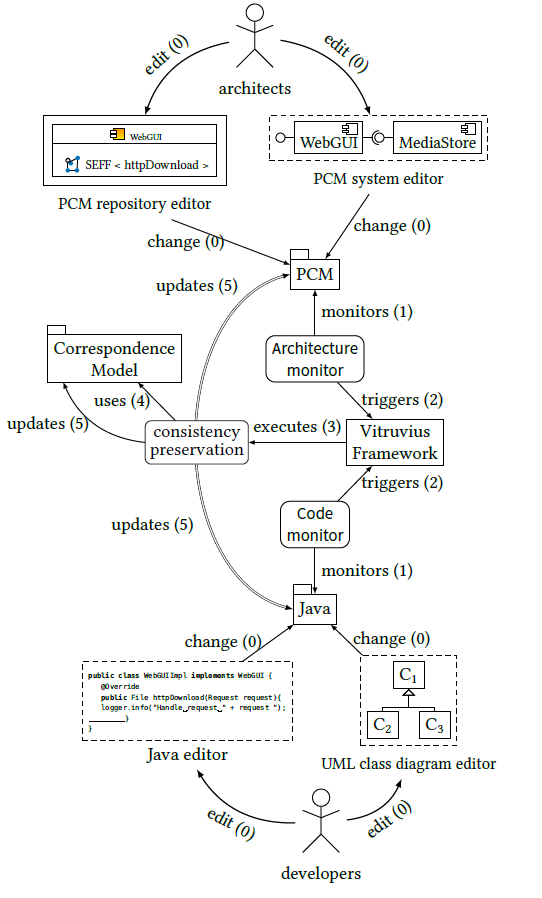
\includegraphics[width=0.9\textwidth]{figures/coevolution_approach}
\caption{The steps used in co-evolution approach to keep architecture models and the source code consistent \cite{langhammer2015co}}
\label{fig:coevoloution approach}
\end{figure}

\subsection{Incremental SEFF Reconstruction}
\label{sec:Incremental SEFF Reconstruction}
Langhammer has proposed in his Co-evolution approach an incremental SEFF reconstruction approach Figure \ref{fig:seff incremental reconst} which can build the SEFFs for only the changed parts of the source code. In contrast to SoMoX, the incremental SEFF reconstruction neither require the parsing of the complete project source code nor the SCDM. Moreover, the SEFF of the smallest unit that can be currently incrementally reconstructed is the SEFF of a method. 

The incremental SEFF reconstruction is integrated in the co-evolution approach that means it can use functionalities and information provides by Vitruvius. Moreover, the incremental SEFF reconstruction is done in change-driven way, that means change that happened in the source code are captured in a Vitruvius change model instance and can be treated in order to regenerate the SEFF of the method in which they belong. To classify the method calls which is necessary for SEFF reconstruction, Langhammer uses the current preservation rules and information from the Vitruvius correspondence model. More details on this step can be found in his thesis \cite{langhammer2017automated}.

\begin{figure}[h]
\centering
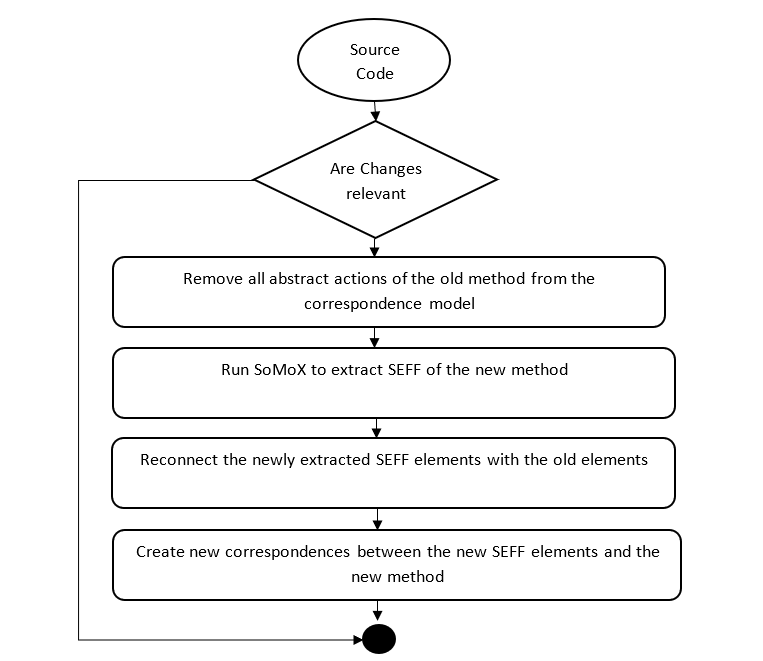
\includegraphics[width=0.9\textwidth]{figures/inscremental_seff_reconst}
\caption{Overview of the incremental reconstruction process of SEFF}
\label{fig:seff incremental reconst}
\end{figure}


\section{Kieker Monitoring Framework}
\label{sec:Kieker Monitoring}
Kieker is an extensible Java-based application performance monitoring and dynamic software analysis framework \cite{van2009continuous}. Figure \ref{fig:kieker} shows the architecture of Kieker framework. It's composed from two main components, namely the monitoring component and analysis component.   The analysis component can be used to read monitoring data, analyze and visualize them for a certain purpose, like generating UML sequence diagram, dependency graphs or Markov chains.

The monitoring component is responsible for source code instrumentation, data collection and data logging. The Monitoring probes are responsible for collecting the monitoring data and send them to the monitoring controller component, which instantiates a monitoring record for every probe. The Monitoring writer component receives the monitoring records from the monitoring controller and serialize them to the monitoring log/stream. 

A monitoring Record represents the measurement data gathered in a single measurement. Kieker provides the possibility to store different types of records for different types of probes. Kieker offers the possibility to create customized probes. We can create new probes either manually by extending the interface IKiekerMonitoringProbe or automatically by using the Instrumentation Record Language (IRL) \cite{jung2013instrumentation}. For example, in one record, we can store the signature and the response time of a method, in another record, we can persist the response time of specific number of statements inside a method.

A monitoring Probe represents the monitoring logic used to collect measurement data from the application. There are two ways to use probe within Kieker.  There is the manually instrumentation, which consists of mixing the instrumentation logic with the business logic of the application. Figure \ref{lst:kieker_manual_instr} show an example, in which the monitoring probe is implemented by mixing monitoring logic with business logic, in this example we create a probe that logs the name of the called service, the start time and end time. Kieker includes also probes based on Aspect Oriented Programming (AOP) \cite{kiczales1997j}, which helps to separates the instrumentation logic from the business logic. Kieker defines AOP based monitoring probes like OperationExecutionAspectAnnotation and OperationExecutionAspectAnnotationServlet. Figure \ref{lst:kieker_aop_instr} shows how the instrumentation looks like, when using AOP for probes implementation.

Using AOP to instrument the source code has the advantage of separating concerns. However, this technique has a limitation, when it comes to the monitoring of certain statements of inside a method, like monitoring the number of executions of a loop or the probability of a branch execution, because the annotation possibilities on these cases are out of box. 


\begin{figure}[h]
\centering
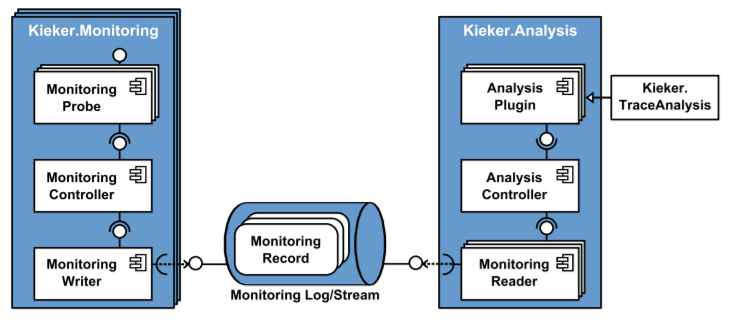
\includegraphics[width=0.9\textwidth]{figures/kieker}
\caption{Overview of the Kieker's architecture \cite{van2009continuous}}
\label{fig:kieker}
\end{figure}

\begin{lstlisting}[caption={Example of manual instrumentation of source code},label={lst:kieker_manual_instr}, captionpos=b, language=java] 
    final long tin = MONITORING_CONTROLLER.getTimeSource().getTime();
    // call of the service
    this.serviceA();
    final long tout = MONITORING_CONTROLLER.getTimeSource().getTime();
     // Create a new record and set values
    final MyResponseTimeRecord e = new MyResponseTimeRecord(
    "serviceA", tout, tin);
    // Pass the record to the monitoring controller
    MONITORING_CONTROLLER.newMonitoringRecord(e);
\end{lstlisting}


\begin{lstlisting}[caption={Example of a Kieker Probe using AOP},label={lst:kieker_aop_instr}, captionpos=b, language=java] 
    @OperationExecutionMonitoringProbe
    public void serviceA(){
       /*
        method content
       */
    }
\end{lstlisting}


\section{Source Code Model eXtractor}
\label{sec:Source Code Model eXtractor}
Source Code Model eXtractor (SoMoX) is a reverse engineering approach, which has been developed by Krogmann \cite{krogmann2012reconstruction}. SoMoX is able to reverse-engineer software component architectures. Moreover, SoMoX can extract a PCM repository from source code and creates a PCM system derived from the repository. The repository created by SoMoX contains mainly components, interfaces, roles and SEFFs. Thus, the results of reverse engineering of SoMoX depend strongly on the project implementation to reverse-engineer which means that SoMoX delivers best results, if the analyzed source code followed a component-based architecture.

In the following, we will review only the features of SoMoX that are involved in the context of this thesis. 

In order to create the architecture of a software system, SoMoX reverse-engineer the software system using the following steps:
\begin{itemize}
\item Parse the source code into a model.  
\item Detect components and interfaces using metrics.
\item Detect data types and signatures using metrics.
\item Reconstruct the SEFFs.
\end{itemize}

For the source code parsing in the first step, SoMoX uses JaMoPP to create an EMF model of the Java source code that can be manipulated. In this thesis, we will also use JaMoPP source code parsing and manipulation purpose.

For components and interfaces detection, SoMoX uses various source code metrics and combine them to determine detection strategies for architecture elements. These metrics must be given each a value between 0 and 100 by the user of SoMoX. The value of the metric tells SoMoX the impact factor, for example the value 0 of a metric means that the impact factor is low, whereas the value 100 of the metric means that the impact factor is high. 

The reconstruction of SEFFs which aims to reverse-engineer the statical behaviour of the source code is done by analysing the methods of the source code. This step has been extended by Langhammer \cite{langhammer2017automated} and its results are used in thesis. In the following, we will explain briefly how the reconstruction of SEFFs is done within SoMoX and how it was extended by Langhammer.
\subsection{Source Code Decorator Model}
\label{sec:Source Code Decorator Model}

The Source Code Decorator Model (SCDM) has been presented within the SoMoX approach (Section \ref{sec:Source Code Model eXtractor}).  SoMoX reverse-engineers the source code and can extracts the architecture models from it. Moreover, SoMoX can be used to extract the Palladio Component Model (PCM) from the Java Source Code. The SCDM is used to create trace links at the model level. The linking between the source code elements and the architecture model elements are needed in the reverse-engineering process. Therefore, the SCDM creates links between the source code elements and the PCM elements. Furthermore, due to the use of SCDM, the reverse-engineering process can be done without mixing the linking concerns with the domain specific language of the source code model and the architecture model.

The SCDM was also used in the Coevolution approach (Section \ref{sec:Automated Coevolution of Source Code and Software Architecture Models}) which keeps automatically the Java Source Code and the PCM models consistent during the system development. The SCDM was used to contain the information, which source code element is reverse-engineered into which architectural model element. For example, it contains the information, which classes are mapped into which component.

In our approach we will need the SCDM in order to map between the SEFF elements and the source code elements or the statements. As mentioned before, the instrumentation points in our approach are represented by the SEFF elements. Moreover, in order to insert the instrumentation code in the right location in the source code of the system, we need to know which SEFF elements corresponds to which source code statements. The SCDM offers this possibility by mapping between each SEFF element and the corresponding JaMoPP statements. 

In order to map between the SEFF elements and the JaMoPP statements, we do not need to implement this feature because it's done already in the Incremental SEFF Reconstruction Process (section \ref{sec:Incremental SEFF Reconstruction}) in the Coevolution approach. This process can monitor the changes within the source code and reconstructs incrementally the SEFF models. Moreover, the execution of this process requires the execution of the SoMoX in order to reverse-engineer the changed parts of the source code. The execution of SoMoX creates the SCDM which maps between the SEFF elements (like Branch Actions, Internal Actions, etc.) and the JaMoPP statements Figure \ref{fig:seff jamopp}.


\begin{figure}[h]
\centering
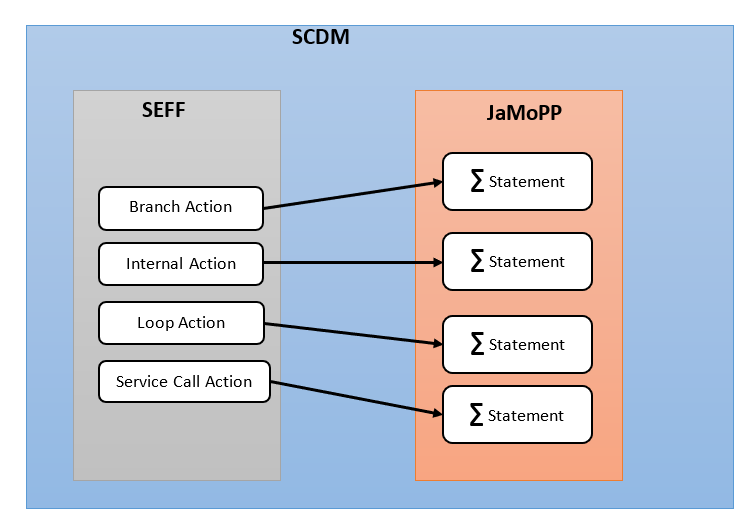
\includegraphics[width=0.9\textwidth]{figures/seff_jamopp}
\caption{Source Code Decorator Model (SCDM) maps between the SEFF elements and the corresponding JaMoPP statements}
\label{fig:seff jamopp}
\end{figure}

\subsection{SoMoX SEFFs Reconstruction}  
\label{sec:SoMoX SEFFs Reconstruction}
For SoMoX SEFFs reconstruction which is done in the last step of the reverse-engineering process, SoMoX uses two models which were created in the first and the second steps. The first model is the Java source code model which was created in the first step and the second is the so-called Source Code Decorator Model (SCDM) which was created in the second step. The SCDM contains the information that map between the source code model elements and the reverse-engineered architectural model elements.

In order to create the SEFF of a method, SoMoX analyses the source code of the method which was detected as a provided method of a component. This analysis is performed in two steps which are described in the following.

In the first step, the SoMoX visits all the method calls within the analysed method and classified them in three categories. The first category contains the component-external method calls which are considered as required roles. The second category contains library calls which considered as calls to a third-party library like java.lang. the second category contains the component-internal calls which are calls to the inner methods of the component. 

In the second step, SoMoX creates the SEFF for the method.  To do so, SoMoX visit again the statements in the source code of the method in order to find the following SEFF elements if they exist: ExternalCallActions, BranchActions, LoopActions and InternalActions. BranchActions and LoopActions are created for branches and loops. A Branch or a Loop is considered as BranchAction or LoopAction if it has an external method call, else it will be combined with an InternalAction.

\section{DevOps}
\label{sec:DevOps}
DevOps \cite{brunnert2015performance} is an agile development process which combines between development (Dev) and operations (Ops). The main goal of DevOps is to reduce the time between changes in the business process and the delivery of a solution to these changes. It achieves its goal by acting mainly on simplifying the communication between organizational and technical teams as well as introducing the automatization for the tasks that can be automated. 

\section{Continuous Integration of Performance Model}
\label{sec:Continuous Integration of Performance Model}
Continuous Integration of Performance Model (CIPM) is an approach proposed by Mazkatli and Koziolek \cite{mazkatli2018continuous} in order to extract incrementally and iteratively the Performance Model from the source code and enrich it by the Performance Model Parameters (PMPs). Furthermore, CIPM aims to keep the source code and the extracted Performance Model consistent during the system development. CIPM extends the Continuous Integration (CI) and the Continuous Deployment (CD) of the source code with a continuous integration of the performance model. 

To achieve that Mazkatli and Koziolek used the Coevolution approach developed by Langhammer (Section \ref{sec:Automated Coevolution of Source Code and Software Architecture Models}) which uses the Palladio Performance Model as a Performance Model and the Vitruvius Platform to keep incrementally and in a change-driven way the source code and the corresponding Performance Model consistent. CIPM uses likewise a change-driven way to enrich the extracted PM by the Coevolution process with PMPs. It defines the consistency rules that minimize the monitoring of the source code execution and the analysis overhead. In addition, it specifies a self-validation process that validates the estimated PMPs. To release that, CIPM automates four activities that are executed in each iteration \ref{fig:CIMP activities}. In this section we will describe only the first two activities because we based our work on them, more details on the other activities can be found in \cite{mazkatli2018continuous}.

The activities in CIPM are represented by the Reaction Language (RL) routines. RL is used in Vitruvius to describe the consistency rules and it's based on two concepts, namely reaction and routine. A reaction specifies changes and triggers a routine that contains the consistency rules that should be executed in reaction to these changes.  

The first activity in CIPM is responsible for updating the structure of the performance model, the usage model and the probes used in the activity two. The structure of the performance model is updated based on the work of Langhammer \cite{langhammer2015co}. The usage model is extracted incrementally from the test cases. For the probes generation CIPM specifies an Instrumentation Metamodel (IMM) and added it to VSUM. IMM contains and manages the instrumentation points and the weaving information based on Aspect-oriented Programming (AOP) \cite{kiczales1997j}. CIMP defines the consistency rules that keep the instrumentation model and the source code consistent. For example, a new probe can be added to the instrumentation model, when a part of the source code was added that corresponds to a new SEFF element. 

The second activity uses the probes from the first activity, instruments the source code and creates the monitoring data. For the monitoring data, CIPM specifies a Measurement Meta-model (MMM) and added it to VSUM. MMM describes the data structures of the different monitored data as well as the consistency rules to keep it consistent with the IMM. For example, after the monitoring phase is done, if a SEFF element had enough monitoring data, this element has to be deactivated in the instrumentation model. 

\begin{figure}[h]
\centering
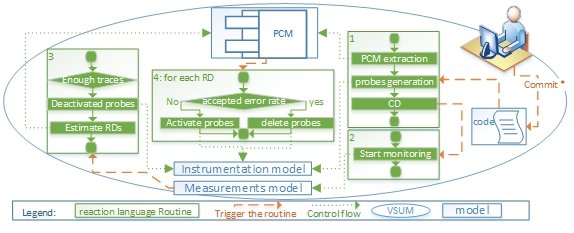
\includegraphics[width=0.9\textwidth]{figures/cipm}
\caption{CIMP activities \cite{mazkatli2018continuous}}
\label{fig:CIMP activities}
\end{figure} 

\subsection{Iterative Performance Model Parameter Estimation Considering Parametric Dependencies}
\label{sec:Iterative Performance Model Parameter Estimation Considering Parametric Dependencies}
Jägers has created his master thesis \cite{jagers2018Iterative} an approach that can estimate Performance Model Parameters taking into account the parametric dependencies. The approach is based on the vision presented by Mazkatli and Koziolek (Section \ref{sec:Continuous Integration of Performance Model}), it extends precisely the concepts introduced in the activities three and four in Figure \ref{fig:CIMP activities}. The approach is designed to make iteratively the estimation and thus reduce the overhead resulting from the estimation for the whole system. 

Jan uses the Palladio Performance model as a Performance Model for his approach. Since the Palladio Performance Model is expressed in terms of SEFF, Jan estimates the performance model parameters for loop iteration, resource demands, branch transitions and external call arguments. He specifies diverse predictive models for estimating Performance model parameters. He uses decision threes to create a predictive model for branch transitions. For loop iterations and resource demands he uses regression analysis. The predictive models are related with service call arguments. The predictive models can be transformed into stochastic expressions in order to use them for enriching performance model.

This approach uses as inputs the monitoring data that are generated from instrumenting and executing the source code that corresponds to the performance mode for which the estimation is done. The monitoring data are structured in records that contain diverse information about diverse source code elements like loop record, branch record response time record etc. Since the execution depends strongly on the monitoring data, in order to keep the estimation iterative, the monitoring must be also done iteratively. this includes also the fine-grained, automatic, iterative instrumentation of the source code. the instrumentation has to be fine-grained because the estimation requires specific information about the program elements like the number of loop execution, the response time of a specific source code that corresponds to an internal action. This thesis provides an approach that can generate iteratively the monitoring data for performance model. These monitoring data can be used by the approach of Jan to make the estimations.







